\begin{frame}[plain]
\begin{center}
\Huge{Examples}
\end{center}
\end{frame}

\begin{frame}
\frametitle{Typical steps}

Write Julia code not an input file.

Typical steps:
\begin{itemize}
\item Initialize Atoms
\item Initialize Hamiltonian with the given Atoms
\item Solve the Hamiltonian
\end{itemize}

Atomic units are used (energy: Hartree, length: bohr)

\end{frame}


\begin{frame}[fragile]
\frametitle{Example: hydrogen molecule in a box}

{\centering
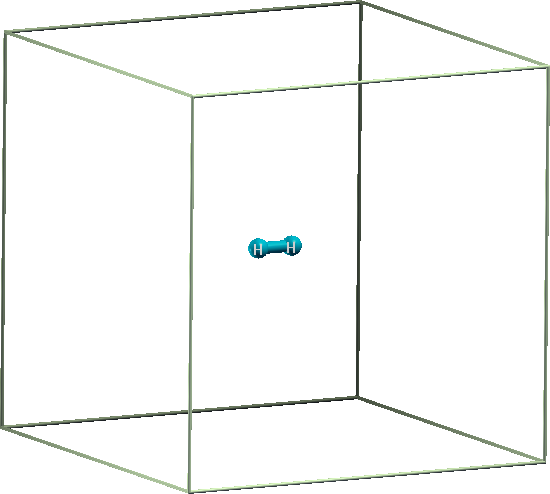
\includegraphics[width=0.25\textwidth]{codes/H2/H2.png}

}

\begin{juliacode}
using PWDFT # activate PWDFT package

# Initialize an H2 molecule in cubic box (simple cubic lattice)
# The coordinates are read from
atoms = Atoms( xyz_file="H2.xyz",
               LatVecs=gen_lattice_sc(16.0) )

pspfiles = ["H-q1.gth"] # pseudopotential parameters

ecutwfc = 15.0 # cutoff energy for wave function expansion

# initialize Hamiltonian
Ham = Hamiltonian( atoms, pspfiles, ecutwfc )

# solve the Kohn-Sham problem (using SCF algorithm)
KS_solve_SCF!( Ham )
\end{juliacode}


\end{frame}


\begin{frame}[fragile]
\frametitle{Output}

\begin{textcode}
$ julia run.jl 

Self-consistent iteration begins ...
update_psi = LOBPCG
mix_method = simple
Density mixing with betamix =    0.20000
    
-------------------------------------------------------
       iter            E            ΔE           Δρ
-------------------------------------------------------
SCF:     1      -0.9088890376  9.08889e-01  1.36287e-04
SCF:     2      -0.9197780666  1.08890e-02  1.17877e-04
SCF:     3      -0.9589404606  3.91624e-02  9.53668e-05
SCF:     4      -0.9975511159  3.86107e-02  7.60953e-05
.... # snipped
\end{textcode}

\end{frame}


\begin{frame}[fragile]
\frametitle{Converged Kohn-Sham energy components}

\begin{columns}[T]

\begin{column}{0.45\textwidth}
PWDFT.jl's result:
\begin{textcode}
-------------------------
Final Kohn-Sham energies:
-------------------------

Kinetic    energy:       1.0100082069
Ps_loc     energy:      -2.7127851088
Ps_nloc    energy:       0.0000000000
Hartree    energy:       0.9015229089
XC         energy:      -0.6314259148
PspCore    energy:      -0.0000012675
-------------------------------------
Electronic energy:      -1.4326811753
NN         energy:       0.3131700043
-------------------------------------
Total      energy:      -1.1195111709
\end{textcode}
\end{column}

\begin{column}{0.55\textwidth}

ABINIT's result:
\begin{textcode}
Components of total free energy (in Hartree) :

   Kinetic energy  =  1.01004059294567E+00
   Hartree energy  =  9.01545039301481E-01
   XC energy       = -6.31436384237843E-01
   Ewald energy    =  3.13170052325859E-01
   PspCore energy  = -1.26742500464741E-06
   Loc. psp. energy= -2.71283243086241E+00
   NL   psp  energy=  0.00000000000000E+00
   >>>>>>>>> Etotal= -1.11951439795224E+00
\end{textcode}
\end{column}

\end{columns}

\end{frame}